\usepackage[shortlabels]{enumitem}
\usepackage{amsmath,amsfonts,amssymb}
\usepackage{latexsym}
\usepackage{gensymb}
\usepackage{mathtools}

\usepackage{amsthm}

% nice fonts
\usepackage{libertine}
\usepackage[libertine,vvarbb]{newtxmath}
\usepackage[scaled=0.96]{zi4}
\DeclareMathAlphabet{\mathcal}{OMS}{cmsy}{m}{n}

% nice links
\usepackage{xcolor}
\usepackage[colorlinks, linkcolor=purple, citecolor=blue!75!black, urlcolor=purple]{hyperref}
\usepackage[noabbrev,capitalise]{cleveref}

% has to be after cleveref
\newtheorem{theorem}{Theorem}
\newtheorem{lemma}[theorem]{Lemma}
\newtheorem{fact}[theorem]{Fact}
\newtheorem{proposition}[theorem]{Proposition}
\newtheorem{corollary}[theorem]{Corollary}
\newtheorem{definition}[theorem]{Definition}
\newtheorem{claim}[theorem]{Claim}
\newtheorem{example}[theorem]{Example}

\makeatletter
% superimpose two math symbols
\newcommand{\superimpose}[2]{{%
  \ooalign{%
    \hfil$\m@th#1\@firstoftwo#2$\hfil\cr
    \hfil$\m@th#1\@secondoftwo#2$\hfil\cr
  }%
}}
\makeatother

\newcommand*{\tensor}{\otimes}
\newcommand*{\mat}[1]{\begin{bmatrix}#1\end{bmatrix}}
\newcommand*{\tp}[0]{\mathsf{T}}
\renewcommand*{\iff}[0]{\leftrightarrow}
\renewcommand*{\emptyset}[0]{\varnothing}
\newcommand{\dotcup}[0]{\mathbin{\mathpalette\superimpose{{\cdot}{\cup}}}}
\DeclareMathOperator*{\bigdotcup}{\mathpalette\superimpose{{\cdot}{\bigcup}}}
\newcommand*{\poly}{\mathsf{poly}}
\newcommand*{\E}{\mathbf{E}}
\DeclareMathOperator*{\Var}{\mathrm{Var}}
\DeclareMathOperator*{\Cov}{\mathrm{Cov}}
\DeclareMathOperator*{\esssup}{ess\,sup}
\DeclareMathOperator*{\essinf}{ess\,inf}
\DeclarePairedDelimiter{\norm}{\lVert}{\rVert}
\DeclarePairedDelimiter{\floor}{\lfloor}{\rfloor}
\DeclarePairedDelimiter{\ceil}{\lceil}{\rceil}
\newcommand*{\C}{\mathbb{C}}
\newcommand*{\F}{\mathbb{F}}
\newcommand*{\N}{\mathbb{N}}
\newcommand*{\Q}{\mathbb{Q}}
\newcommand*{\R}{\mathbb{R}}
\newcommand*{\Z}{\mathbb{Z}}

\def\[#1\]{\begin{align*}#1\end{align*}}
\newcommand*{\aln}[1]{\begin{aligned}#1\end{aligned}}
\newcommand*{\pheq}{\mathrel{\phantom{=}}} % invisible = for align mode
\newcommand*{\mmid}{\mathrel{}\middle|\mathrel{}}

\newcommand*{\defn}[1]{\textbf{\textit{\boldmath #1}}}

\newcommand*{\eqdef}[0]{\mathrel{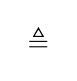
\begin{tikzpicture}[scale=0.06,baseline={(e.south)}]
      \draw (0, 0) -- (1, {-sqrt(3)}) -- (-1, {-sqrt(3)}) -- cycle;
      \node[anchor=base,inner sep=0pt] (e) at (0, -5) {$=$};
\end{tikzpicture}}}
